\documentclass[a4paper,12pt]{article}
\usepackage[english]{babel}
\usepackage[utf8]{inputenc}
\usepackage{setspace}

% Larger borders -- we do not want do waste paper, even if it is only paper on screen =)
\usepackage[top=2.5cm, bottom=2.5cm, left=2cm, right=2cm]{geometry}
% Remove auto indentation of paragraphs.
\setlength\parindent{0pt}

% Palatino font (nicer serif font: Times is for oldies)
\renewcommand*\rmdefault{ppl}

% Nested itemize list bullet style
\renewcommand{\labelitemi}{$\bullet$}
\renewcommand{\labelitemii}{$\circ$}
\renewcommand{\labelitemiii}{--}

% Math packages
\usepackage{mathtools}
\usepackage{amsmath}
\usepackage{amsfonts}
\usepackage{amssymb}

% Graphic packages
\usepackage{graphicx}
\usepackage{float}
\usepackage{adjustbox}
\usepackage{tikz}
\usepackage{forest,array}
\usetikzlibrary{shadows}

% Graphs styles
\forestset{
  giombatree/.style={
    for tree={
      grow = east,
      parent anchor=east,
      child anchor=west,
      edge={rounded corners=2mm},
      fill=violet!5,
      drop shadow,
      l sep=10mm,
      edge path={
        \noexpand\path [draw, \forestoption{edge}] (!u.parent anchor) -- +(5mm,0) -- (.child anchor)\forestoption{edge label};
      }
    }
  }
}
\forestset{
  qtree/.style={
    for tree={
      parent anchor=south,
      child anchor=north,
      align=center,
      edge={rounded corners=2mm},
      fill=violet!5,
      drop shadow,
      l sep=10mm,
    }
  }
}

% BAN logic macros
\newcommand{\believes}{\mid\!\equiv}
\newcommand{\sees}{\triangleleft}
\newcommand{\oncesaid}{\mid\!\sim}
\newcommand{\controls}{\Rightarrow}
\newcommand{\fresh}[1]{\#(#1)}
\newcommand{\combine}[2]{{\langle #1 \rangle}_{#2}}
\newcommand{\encrypt}[2]{{ \{ #1 \} }_{#2}}
\newcommand{\sharekey}[1]{\xleftrightarrow{#1}}
\newcommand{\pubkey}[1]{\xmapsto{#1}}
\newcommand{\secret}[1]{\xleftrightharpoons{#1}}

\newcommand{\projectname}{Cybersec.proj}

% Hides ugly links from the index
\usepackage[hidelinks]{hyperref}
% Landscape format pdf pagess
\usepackage{pdflscape}


\begin{document}
\pagenumbering{gobble}

{\setstretch{1.0}
  \begin{titlepage}
  	\centering
  	
\includegraphics[width=6cm]{img/unipi.eps}\par
    \vspace{1.5cm}
    {\Large Department of Information Engineering \par}
  	\vspace{1.5cm}
  	{\huge\textsc{Secure FTP application}\par}
  	\vspace{2cm}
  	Francesco \textsc{Barbarulo}\par
  	Bruk Tekalgne \textsc{Gurmesa}\par
    Giovan Battista \textsc{Rolandi}

  	\vfill

    % Bottom of the page
  	{\large A.Y. 2018-2019\par}
  \end{titlepage}
}


\clearpage
~
\clearpage
\tableofcontents
\clearpage
~
\clearpage
\pagenumbering{arabic}

\section{Introduction}
\projectname{} is a client-server application which allows to download and upload files on a server in a secure manner.

\section{Application}
\subsection{Requirements}
\begin{itemize}
  \item a Unix-like environment;
  \item the GNU Compiler Collection Toolchain, any C++11 compliant version;
  \item GNU make;
  \item OpenSSL 1.1.1;
  \item LaTeX suite (optional, for documentation);
\end{itemize}

\subsection{Compile}
To compile the application, just run:
\begin{verbatim}
  $ cd $REPO
  $ make
\end{verbatim}

Application's two executables, \texttt{client} and \texttt{server}, will be found in the \texttt{bin} directory.
For simplicity, it is suggested to run them from the repository's root directory.

To compile this documentation, just run:
\begin{verbatim}
  $ cd $REPO/doc
  $ make
\end{verbatim}

\subsection{Run}
To run the application just type the following commands in your shell.

To run the server's executable:
\begin{verbatim}
  $ bin/server <port>
\end{verbatim}
where
\begin{itemize}
  \item \texttt{port} is the TCP port you want the server to listen for client's connections;
\end{itemize}

To run the client's executable:
\begin{verbatim}
  $ bin/client <IPv6> <port> <username>
\end{verbatim}
where
\begin{itemize}
  \item \texttt{IPv6} is the server's IP address, in IPv6 form; examples of valid addresses are:
  \begin{itemize}
    \item \texttt{::1}
    \item \texttt{2001:470:c844::20}
    \item \texttt{::193.70.88.212}
  \end{itemize}
  \item \texttt{port} is the server's TCP port it listens for client's connections;
  \item \texttt{username} is the user name, that must match the certificate's name in \texttt{cert} directory;
\end{itemize}

\subsection{Usage}
To get a list of usable commands on the client's shell, just type:
\begin{verbatim}
> help
\end{verbatim}

Client's shell accepts the following, self explaining, commands:
\begin{verbatim}
 help           -- show this content
 rls            -- list remote files
 lls [<path>]   -- list local files
 get <filename> -- download the specified remote file
 put <filename> -- upload the specified local file
 rm <filename>  -- remove the specified remote file
 q              -- quit
\end{verbatim}

\subsection{Repository}
\projectname{}'s repository is organized in directories:
\begin{itemize}
  \item \texttt{bin} contains the \texttt{client} and \texttt{server} executable files;
  \item \texttt{cert} contains all the certificates; if the application's server is run on the same host as the client, then this directory can be shared.
  \item \texttt{conf} contains server configuration, eg. a file with authorized clients list;
  \item \texttt{debug} contains some useful commands and configuration files for some common debugging tools like \emph{valgrind} and \emph{gdb};
  \item \texttt{doc} contains the \LaTeX source code of this document;
  \item \texttt{downloads} is the default location for files downloaded from the server by the client;
  \item \texttt{obj} contains object files before their linking;
  \item \texttt{root} is the default and only location allowed for files uploaded to the server;
  \item \texttt{src} contains the application's source code;
\end{itemize}

\subsubsection{\texttt{cert} directory}
\begin{itemize}
    \item \texttt{\emph{username}\_cert.pem} and \texttt{\emph{username}\_key.pem} contains \emph{username}'s certificate and private key, respectively, in PEM format;
    \item \texttt{TrustedCA\_cert.pem} and \texttt{TrustedCA\_crl.pem} contains the trusted public certification authority's certificate and certificate revocation list, in PEM format;
\end{itemize}

Repository contains a basic configuration with an example \texttt{TrustedCA\_cert.pem} and \texttt{TrustedCA\_crl.pem} certificate and certificate revocation list, and the following user's certificates:
\begin{figure}[H]
\centering
\begin{tabular}{| l | c | c | c |}\hline
username  & signed by TrustedCA & revoked & authorized user \\ \hline
alice     & yes                 & no      & yes             \\ \hline
bob       & yes                 & no      & no              \\ \hline
charlie   & yes                 & yes     & yes             \\ \hline
server    & yes                 & no      & no              \\ \hline
trudy     & no                  & --      & no              \\ \hline
\end{tabular}
\end{figure}

\subsubsection{\texttt{src} directory}
\begin{itemize}
  \item \texttt{client} contains client's application source code;
  \item \texttt{common} contains application's utilities modules and interface layer for OpenSSL;
  \item \texttt{server} containts server's application soruce code;
\end{itemize}

\subsection{Debug mode}
To compile application with debug symbols and log, run:

\begin{verbatim}
  $ make DEBUG=true
\end{verbatim}

and then run the executables passing one of these magic words as the last parameter:

\begin{itemize}
  \item \texttt{FATAL} or \texttt{ERROR}: show only fatal errors;
  \item \texttt{WARNING}: shows also warnings, useful to exploit unexpected behaviors or detect intrusion attempts;
  \item \texttt{INFO}: shows a lot of verbose information to deeply inspect application's flow;
  \item \texttt{DEBUG}: shows almost every information;
\end{itemize}

Warning: use of debug level \texttt{DEBUG} leads to sensitive data leaks, such as session keys!

\subsection{Modules}
Application is organized in the following modules.

\begin{figure}[H]
  \centering
  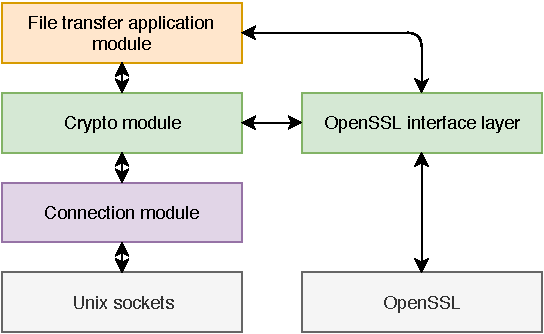
\includegraphics{img/modules.pdf}
  \caption{Application modules}
  \label{img:modules}
\end{figure}

where
\begin{itemize}
  \item \emph{File transfer application} is the actual application which manages file transfers;
  \item \emph{Crypto module} provides send/receive API, and manages traffic security during the session;
  \item \emph{OpenSSL interface layer} provides a human usable C++ interface to OpenSSL's plain C API;
  \item \emph{Connection module} provides a human usable C++ interface with send/receive API for Unix sockets;
\end{itemize}

Since \emph{Connection} module and \emph{Crypto} module provide the same send/receive API to their upper layers, the \emph{Crypto} module can be entirely added, or removed, with only minor changes to the \emph{File transfer application}, to make an application that works in the clear.

\emph{OpenSSL interface} layer is used by the \emph{Crypto} module to manage the session's security, and by the \emph{File transfer application} module to perform the initial handshake.

\section{Network protocol overview}
\projectname{}'s network stack is organized as shown in Figure~\ref{img:protocol}.

\begin{figure}[H]
  \centering
  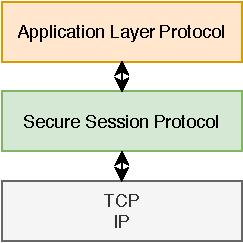
\includegraphics{img/protocol.pdf}
  \caption{Network protocol overview}
  \label{img:protocol}
\end{figure}

\section{Application layer protocol}
Application layer manages its input/output data as continuos infinite stream of bytes.

The application sends and receives request commands, reply statuses, and generic streams of bytes (the body), whose meaning depends on the previous sent/received command/reply.

The protocol partially resembles HTTP.

A \texttt{parola} is defined as a pure ASCII sequence which can match the following regular expression \texttt{[A-Za-z0-9\textbackslash.\_]*}.
Different \texttt{parola}s can be separated by whitespaces.

Every command must be composed of one or more \texttt{parola}s.

\subsection{Request commands}
A request command is sent by the client to the server.

Generic structure of a request command is:
\begin{verbatim}
COMM filename\n
tag: value\n
\n
body
\end{verbatim}

Each line is terminated by a line feed(\texttt{LF}) char, and each command is terminated by a \texttt{LF} char.
It is important to send the \texttt{LF} char because server will not parse the command until two trailing \texttt{LF}s are received.

Note: a \texttt{LF} char is represented by a byte whose value is \texttt{0x0A}.
\\
A command is composed by the following parts:
\begin{itemize}
  \item \texttt{COMM} is a 4 char \texttt{parola} and represents the command to issue;
  \item \texttt{filename} is the name of a file on which issue the command.
  Filenames are composed by one \texttt{parola}.
  Depending on the specific command type, use of a filename is mandatory or forbidden;
  \item \texttt{tag: value} is a pair of two \texttt{parola}s, composed by a \texttt{parola} immediately followed by a colon, a whitespace and another \texttt{parola}.
  First \texttt{parola} represents the tag for an additional parameter of current command, while second one representes the actual value for the parameter; depending on the specific command, one or more parameters may be mandatory or forbidden;
  \item \texttt{body} is a stream of bytes whose length must be specified in a command parameter; depending on the specific command type, use of a body is mandatory or forbidden:
\end{itemize}

\subsection{Reply status}
A reply status is sent by the server to the client.

Generic structure of a reply status is:

\begin{verbatim}
DDD\n
tag: value\n
\n
body
\end{verbatim}

A reply status is composed by the following parts:
\begin{itemize}
  \item \texttt{DDD} a 3 ASCII digits number representing the state of the previous request command;
  \item \texttt{tag: value} is a pair to represent a parameter, with the same format of the request command parameter; depending on the specific command type received, one or more parameters may be mandatory or forbidden;
  \item \texttt{body} is a stream of bytes whose length must be specified in a reply status parameter; depending on the specific command the reply refers to, a body is mandatory or forbidden;
\end{itemize}

\subsection{Request commands list}

\paragraph{DELE}
\texttt{DELE filename}

Reply status:
\begin{itemize}
  \item \texttt{200}: ok
  \item \texttt{452}: bad file
\end{itemize}

\paragraph{LIST}
\texttt{LIST}

Request the server to send a list of available files

Reply status:
\begin{verbatim}
200\n
Size: listsize\n
\n
body
\end{verbatim}

\texttt{body} is a list of \texttt{parola}, each one representing the name of a file and each one separed by a newline.

\paragraph{QUIT}
\texttt{QUIT}

Close connection with the server.

Reply status:
\begin{itemize}
  \item \texttt{200}: ok
\end{itemize}

\paragraph{RETR}
\texttt{RETR filename}

Retrieve a file from the server.

Reply status:
\begin{itemize}
  \item success:
\begin{verbatim}
200\n
Size: filesize\n
\n
body
\end{verbatim}
  \item failure:\\
  \texttt{452}: bad file
\end{itemize}

\paragraph{STOR}
\begin{verbatim}
STOR filename\n
Size: filesize\n
\n
body
\end{verbatim}

Store a file on the remote server, possibly overwriting an existing one.

\begin{itemize}
  \item \texttt{Size: filesize} is a parameter pair. \texttt{filesize} is the decimal ASCII representation of the file size in bytes;
  \item \texttt{body} is the actual content of the file;
\end{itemize}

Reply status:
\begin{itemize}
  \item \texttt{200}: ok
  \item \texttt{452}: bad file
\end{itemize}

\subsection{Generic return values}
\begin{itemize}
  \item \texttt{500}: server error
  \item \texttt{501}: syntax error
  \item \texttt{502}: command not implemented
  \item \texttt{503}: bad sequence of commands
\end{itemize}

\section{Secure layer session protocol}
Every time that the application layer calls the secure layer with new data to send to the other party, a special secure layer packet is created; the receiver then expects to receive the same kind of packet, and extracts data from it to pass to the application level.

Receiver's side transparently checks these packet's validity, and then unfolds them and passes them to the application layer as a stream of bytes.

\begin{figure}[H]
\centering
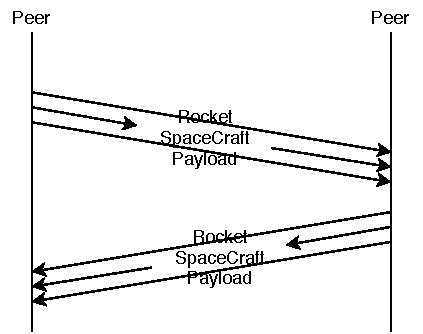
\includegraphics{img/secure-session-protocol.pdf}
\caption{Secure layer session protocol overview}
\label{img:secure-session-protocol}
\end{figure}

\subsection{Secure packets}
Secure packets have two fixed length headers, called \texttt{Rocket} and \texttt{SpaceCraft}.
Every integer has network byte order endianess.

\subsection{Rocket}
First, \texttt{Rocket} is sent (or received).

\begin{verbatim}
struct Rocket {
  unsigned char hmac[HMAC_LEN],
  uint32_t length,
  uint32_t sequence_number
};
\end{verbatim}

where

\begin{itemize}
  \item \texttt{hmac} is used to authenticate \texttt{Rocket}'s content; the hash is computed using the $K_a$ key exchange during the initial handshake;
  \item \texttt{length} is the size, in bytes, of the variable length payload, and it is used to allocate data at receiver's endpoint;
  \item \texttt{sequence\_number} is used to protect against replay attacks;
\end{itemize}

After the \texttt{Rocket}'s content has been authenticated, its content is used to prepare the receiver's buffer.
Then, \texttt{Rocket} can be detached and control passes entirely to \texttt{SpaceCraft}.

\subsection{SpaceCraft}
A \texttt{SpaceCraft} always follows the \texttt{Rocket}.

\begin{verbatim}
struct SpaceCraft {
  unsigned char hmac[HMAC_LEN],
  uint32_t sequence_number
};
\end{verbatim}

where

\begin{itemize}
  \item \texttt{hmac[]} is used to authenticate \texttt{SpaceCraft}'s content, and the encrypted payload;
  \item \texttt{sequence\_number} is used to protect against replay attacks;
\end{itemize}

\subsection{Encrypted Payload}
Finally, the encrypted payload follows the \texttt{SpaceCraft}.

The encrypted payload can be of any length between $0$ and $2^{32}$ bytes, even if in our implementation it has a practical limitation of $4k$ bytes.

The payload is encrypted using AES128 in CFB mode as a stream cipher, in a manner that no padding is required;
encryption is performed using $K_s$ and \emph{iv} exchanged during the initial handshake.

\section{Handshake (key exchange protocol)}
A 3 way handshake is needed in order to establish the secure session.

\begin{figure}[H]
\centering
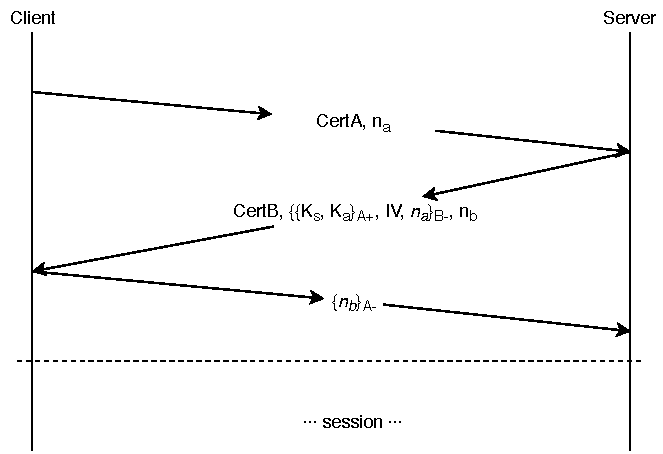
\includegraphics{img/key-exchange-protocol.pdf}
\caption{Key exchange protocol overview}
\label{img:key-exchange-protocol}
\end{figure}

where

\begin{itemize}
  \item \emph{certA} is the Client's certificate; it is signed by a known public trusted certification authority.
  \item $n_a$ is the Client's nonce to challenge the server and protect the communication against replay attacks;
  \item \emph{certB} is the Server's certificate; it is signed by a known public trusted certification authority;
  \item $K_s$, $K_a$ are the two symmetric keys used during the session, to encrypt and to authenticate the data, respectively; they are generated by the Server and transmitted encrypted in an RSA~Seal with Client's public key $A^{+}$;
  \item \emph{iv} is the initialization vector used in conjunction with $K_s$ to initialize the CFB stream cipher, that will be used to encrypt the session;
  \item the encrypted $K_s$, $K_a$, and \emph{iv} and $n_a$, are digitally signed with the Server's private key $B^{-}$;
  \item $n_b$ is the Server's nonce to challenge the client and protect the communication against replay attacks;
  \item italic $n_a$ and $n_b$ in Figure~\ref{img:key-exchange-protocol} indicate that there is no need to actually transmit them on the network, but only their signature is needed;
\end{itemize}

Correctness of the above handshake protocol is proved using BAN logic in the next section.

\subsection{Objectives}

The objectives of the protocol are the key authentication and freshness of the keys:

\[A \believes A \sharekey{k_s, k_a} B \]
\[A \believes \fresh{A \sharekey{k_s, k_a} B} \]

\subsection{Assumptions}

\paragraph{Keys}

\[A \believes \pubkey{CA^+} CA \]
\[B \believes \pubkey{CA^+} CA \]
\[B \believes A \sharekey{k_s, k_a} B \]

\paragraph{Trust}

\[A \believes B \controls A \sharekey{k_s, k_a} B \]
\[A \believes B \controls \fresh{A \sharekey{k_s, k_a} B} \]
\[A \believes CA \controls (cert_A, cert_B) \]
\[B \believes CA \controls (cert_A, cert_B) \]

\paragraph{Freshness}

\[A \believes \fresh{N_A} \]
\[B \believes \fresh{N_B} \]
\[B \believes \fresh{A \sharekey{k_s, k_a} B} \]

\subsection{Idealization}

Since the first message is in clear and the third one is only a challenge response not useful to prove the correctness of the protocol, we will take in account only the second message $M2$ which has the following idealized form:

\[ M2: B \rightarrow A: \{cert_B\}_{CA^-}, \{IV, N_A, \fresh{A \sharekey{k_s, k_a} B}, \{A \sharekey{k_s, k_a} B\}_{A^+}\}_{B^-} \]

\subsection{Proof}

\begin{align}
\frac{A \believes \pubkey{CA^+} CA, A \sees \encrypt{cert_B}{CA^-}}{A \believes CA \oncesaid cert_B} \tag*{postulate 1}
\end{align}

\begin{align}
\frac{A \believes \fresh{certB}, A \believes CA \oncesaid cert_B}{A \believes CA \believes certB} \tag*{postulate 2}
\end{align}
$\fresh{certB}$ is guaranteed by its non-before and not-after validity range.

\begin{align}
\frac{A \believes CA \believes cert_B, A \believes CA \controls cert_B}{A \believes cert_B} \tag*{postulate 3}
\end{align}

$A \believes cert_B$ means that $A \believes \pubkey{B^+} B$, since $\pubkey{B+} B$ is part of $cert_B$.

\begin{align}
\frac{A \believes \pubkey{B^+} B, A \sees \encrypt{payload_{M2}}{B^-}}{A \believes B \oncesaid payload_{M2}} \tag*{postulate 1}
\end{align}

\begin{align}
\frac{A \believes \fresh{payload_{M2}}, A \believes B \oncesaid payload_{M2}}{A \believes B \believes payload_{M2}} \tag*{postulate 2}
\end{align}

Freshness of $payload_{M2}$ is guaranteed by $N_A$.

Since $payload_{M2}$ contains $A \sharekey{k_s, k_a} B$ and $\fresh{A \sharekey{k_s, k_a} B}$, we can state that $A \believes B \believes A \sharekey{k_s, k_a} B$ and $A \believes B \believes \fresh{A \sharekey{k_s, k_a} B}$

\begin{align}
\frac{A \believes B \believes A \sharekey{k_s, k_a} B, A \believes B \controls A \sharekey{k_s, k_a} B}{A \believes A \sharekey{k_s, k_a} B} \tag*{postulate 3}
\end{align}

\begin{align}
\frac{A \believes B \believes \fresh{A \sharekey{k_s, k_a} B}, A \believes B \controls \fresh{A \sharekey{k_s, k_a} B}}{A \believes \fresh{A \sharekey{k_s, k_a} B}} \tag*{postulate 3}
\end{align}

\section{Attack resistance}

The application has been designed to avoid eavesdropping, tampering and message replay attacks. Even the bruteforce attack is not feasible for a nowdays strong adversary.

\subsection{Eavesdropping}
An adversary could want to spy on the client-server conversation. In our implementation the conversation is confidential since we encrypt every message using AES-128-CFB algorithm (shown in Figure~\ref{img:cfb-enc-mode}) offered by OpenSSL library.
Even if the adversary would store every encrypted message, he is not able to decrypt them without knowing the session key.

\begin{figure}[H]
\centering
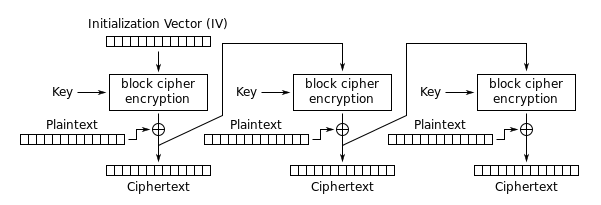
\includegraphics[width=0.8\textwidth]{img/CFB-enc-mode}
\caption{Cipher Feedback encryption mode}
\label{img:cfb-enc-mode}
\end{figure}

% TODO -- if we want to say something more about CFB...

\subsection{Tampering}

An adversary could want to tamper with messages for making the client send unwanted commands such as removing an important file on the server. Fortunately, every session message is authenticated through HMAC which is considered secure. The HMAC is fed with the authentication key, exchanged in the handshake phase, and an adversary can not generate a valid HMAC tag without it. 

\subsection{Message replay}

An adversary could store some messages sent from client A to server B and send them again to make server B think that it is actually talking with client A. This type of attack could make the server act in an unexpected way. Our application foresees that every message is marked with a sequence number. If the expected sequence number does not match the message one, the connection is closed.

Since the sequence number ranges from $0$ to $2^{32} - 1$ it will wrap around after a period of $2^{32}$. As soon as this happens, the parties are not able to distinguish fresh messages from the replay ones anymore. Thus, we force the disconnection from the current session suggesting the reconnection for exchanging new session and authentication keys. 

\subsection{Bruteforce attack}
The last hope for an adversary is represented by the bruteforce attack. The aim of this attack is to find the session key once some plaintext-ciphertext pairs are stored.
Unfortunately for the adversary, the bruteforce attack as a complexity of $O(2^{128})$ for the session key and $O(2^{256})$ for the authentication key.

\end{document}
